\documentclass[mathserif]{beamer}
\usetheme{Berlin} %sidebar
\usecolortheme{dolphin}
\newcommand{\bi}{\begin{itemize}\item}
\newcommand{\ei}{\end{itemize}}
\newcommand{\inner}[2]{\big<\vec{#1}\cdot\vec{#2}\big>}
%\include{../beamer_presentation}


\title{Supervised Learning Linear Priority Dispatch Rules for Job-Shop Scheduling}
\author{Helga Ingimundardottir and Thomas Philip Runarsson}
\date{9. October 2010} % beskidt .. men det virker
\institute{School of Engineering and Natural Sciences, University of Iceland}

%\beamertemplatenavigationsymbolsempty % fjerner pdf-indhold

%\AtBeginSection[]{\begin{frame}<beamer>   \frametitle{Yfirlit}    \tableofcontents[currentsection]  \end{frame} }


%%%%%%%%%%%%%%%%%%%%%%%%%%%%%%%%%%%%%%
\begin{document}
%%%%%%%%%%%%%%%%%%%%%%%%%%%%%%%%%%%%%%
\frame{\titlepage}

\section{Abstract}
\frame{\frametitle{Abstract}
\bi Introduction to a framework in which dispatching rules for \emph{job-shop scheduling problems} (JSSP) are discovered with supervised learning by analyzing characteristics of optimal solutions. 
  \item Ordinal regression implemented to identify good choices from bad at each time step.
  \item Data-driven method.
  \item Robust towards scalability and different data distributions. 
  \item Dispatching rules from this new framework outperform the most common single priority-based dispatching rules w.r.t. minimum makespan. 
  \item Experiments on simulated data. 
\ei
}

\section{Introduction}
\frame{\frametitle{Job Shop Scheduling}
\bi Job shop scheduling consists of a set of $n$ jobs that must be scheduled on a set of $m$ machines. 
 \item Each job consists of a number of operations which are processed on the machines in a predetermined order. 
 \item Optimal schedule is the one where the time to complete all jobs is minimal (minimum makespan).
\ei
}
\frame{\frametitle{Classical methods for solving JSP}
\bi NP hard problem
  \item Solved using ad-hoc dispatching rules. A summary of over 100 dispatching rules used in research can be found in \cite{Panwalkar1977a}.
  \item Most effective single priority based dispatch rules:
  \bi Most work remaining (MWRM)
    \item Least work remaining (LWRM)
    \item Shortest processing time (SPT)
    \item Largest processing time (LPT)
  \ei
\ei
}
\frame{\frametitle{Implementing dispatching rules}
\begin{center}\begin{figure}[H] 
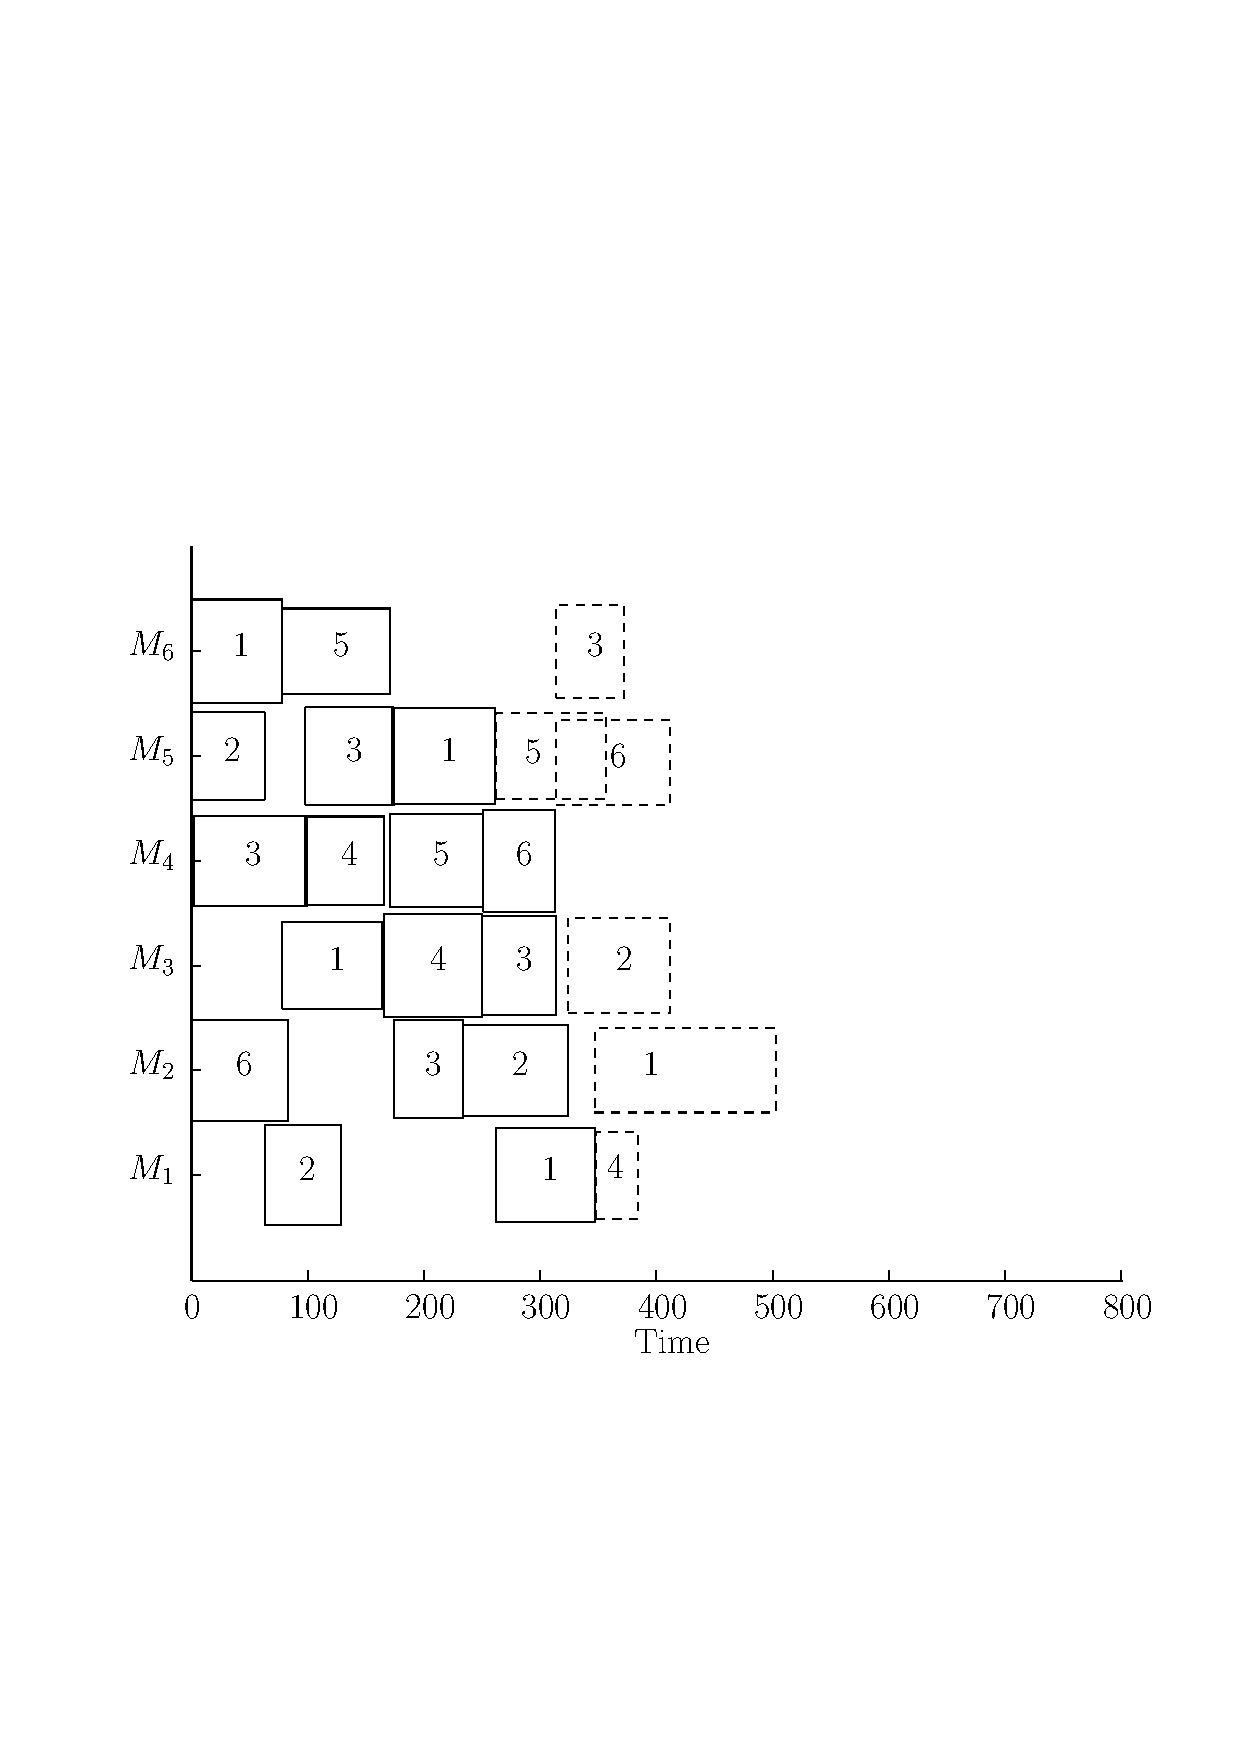
\includegraphics[width=6cm]{dispatch_features.jpg}
\caption{A schedule being built, the dashed boxes represent six different possible jobs that could be scheduled next using a dispatch rule.}
\end{figure}\end{center}
}
\frame{\frametitle{Ordinal regression}
\bi The ranking problem is specified by a set of point/rank
pairs
%\item $Y=\{r_1,\ldots,r_\ell\}$ is the outcome space with ordered ranks $r_1> r_2,> \ldots > r_\ell$.  
\item Mapping of points to ranks: $ \{h(\cdot) : X \mapsto Y\}$
\bi $\vec{x}_i \succ \vec{x}_j \quad \Leftrightarrow \quad h(\vec{x}_i) > h(\vec{x}_j)$ \ei
\item Ordinal regression: obtain function $h^*$ that can for a given pair $(\vec{x}_i,y_i)$ and $(\vec{x}_j,y_j)$ distinguish between two different outcomes: $y_i > y_j$ and $y_j > y_i$. 
\item Problem of predicting the relative ordering of all possible pairs of examples
%\item The training set, composed of pairs, is then as follows: $$S' = \big\{(\vec{x}_k^{(1)}, \vec{x}_k^{(2)}),t_k=\text{sign}(y_k^{(1)} - y_k^{(2)})\big\}_{k=1}^{\ell'}$$ where $(y_k^{(1)} = r_i) \wedge (y_k^{(2)} = r_{i+1})$ (and vice versa) %$(y_k^{(1)} = r_{i+1}) \wedge (y_k^{(2)} = r_{i})$) resulting in $\ell'=2(\ell-1)$ possible adjacently ranked training pairs. 
%\item Rank difference is denoted by $t_k\in[-1,1]$.
\ei
% We deal only in the linear case for now...
%In order to generalize the technique to different point data types and model spaces an implicit kernel-defined feature space with corresponding feature mapping $\phi$ is applied. Consider the feature vector $\phi(\vec{x})=[\phi_1(\vec{x}),\ldots,\phi_m(\vec{x})]^T\in \reals^m$ where $m$ is the number of features. Then the surrogate considered may be defined by a linear function in the kernel-defined feature space: 
The surrogate considered may be defined by a linear function in the feature space:
\begin{equation}  
h(\vec{x}) = \sum_{i=1}^m w_i \vec{x} = \inner{w}{x}. %h(\vec{x}) = \sum_{i=1}^m w_i\phi_i(\vec{x}) = \inner{w}{\phi(\vec{x})}.
\end{equation}

}

\section{Experimental study}
\subsection{Training and test data generation}
\frame{\frametitle{Training and test data generation}
\bi Determine the order (sequence) of jobs assigned, at the first available time slot (to the left)
  \item When job is assigned, new state occurs and features are updated
  \item At each time step, a good/bad ordinal data pair is only created if final makespan is different.
  \bi At least one or more optimal solution for each JSP 
    \item Sequence representation is not uniquely determined.
  \ei
\ei
}

\subsection{Training size and accuracy}
\frame{\frametitle{Training size}
\begin{columns}[t]
\begin{column}{5cm}
\bi Data distributions
 \bi $U(1,100)$
  \item $U(50,100)$
 \ei
 \item Size of data sets:
 \bi Training set: 200
  \item Validation set: 100
  \item Test set: 200
 \ei
\ei
\end{column}
\begin{column}{5cm}
\begin{center}\begin{figure}[H] 
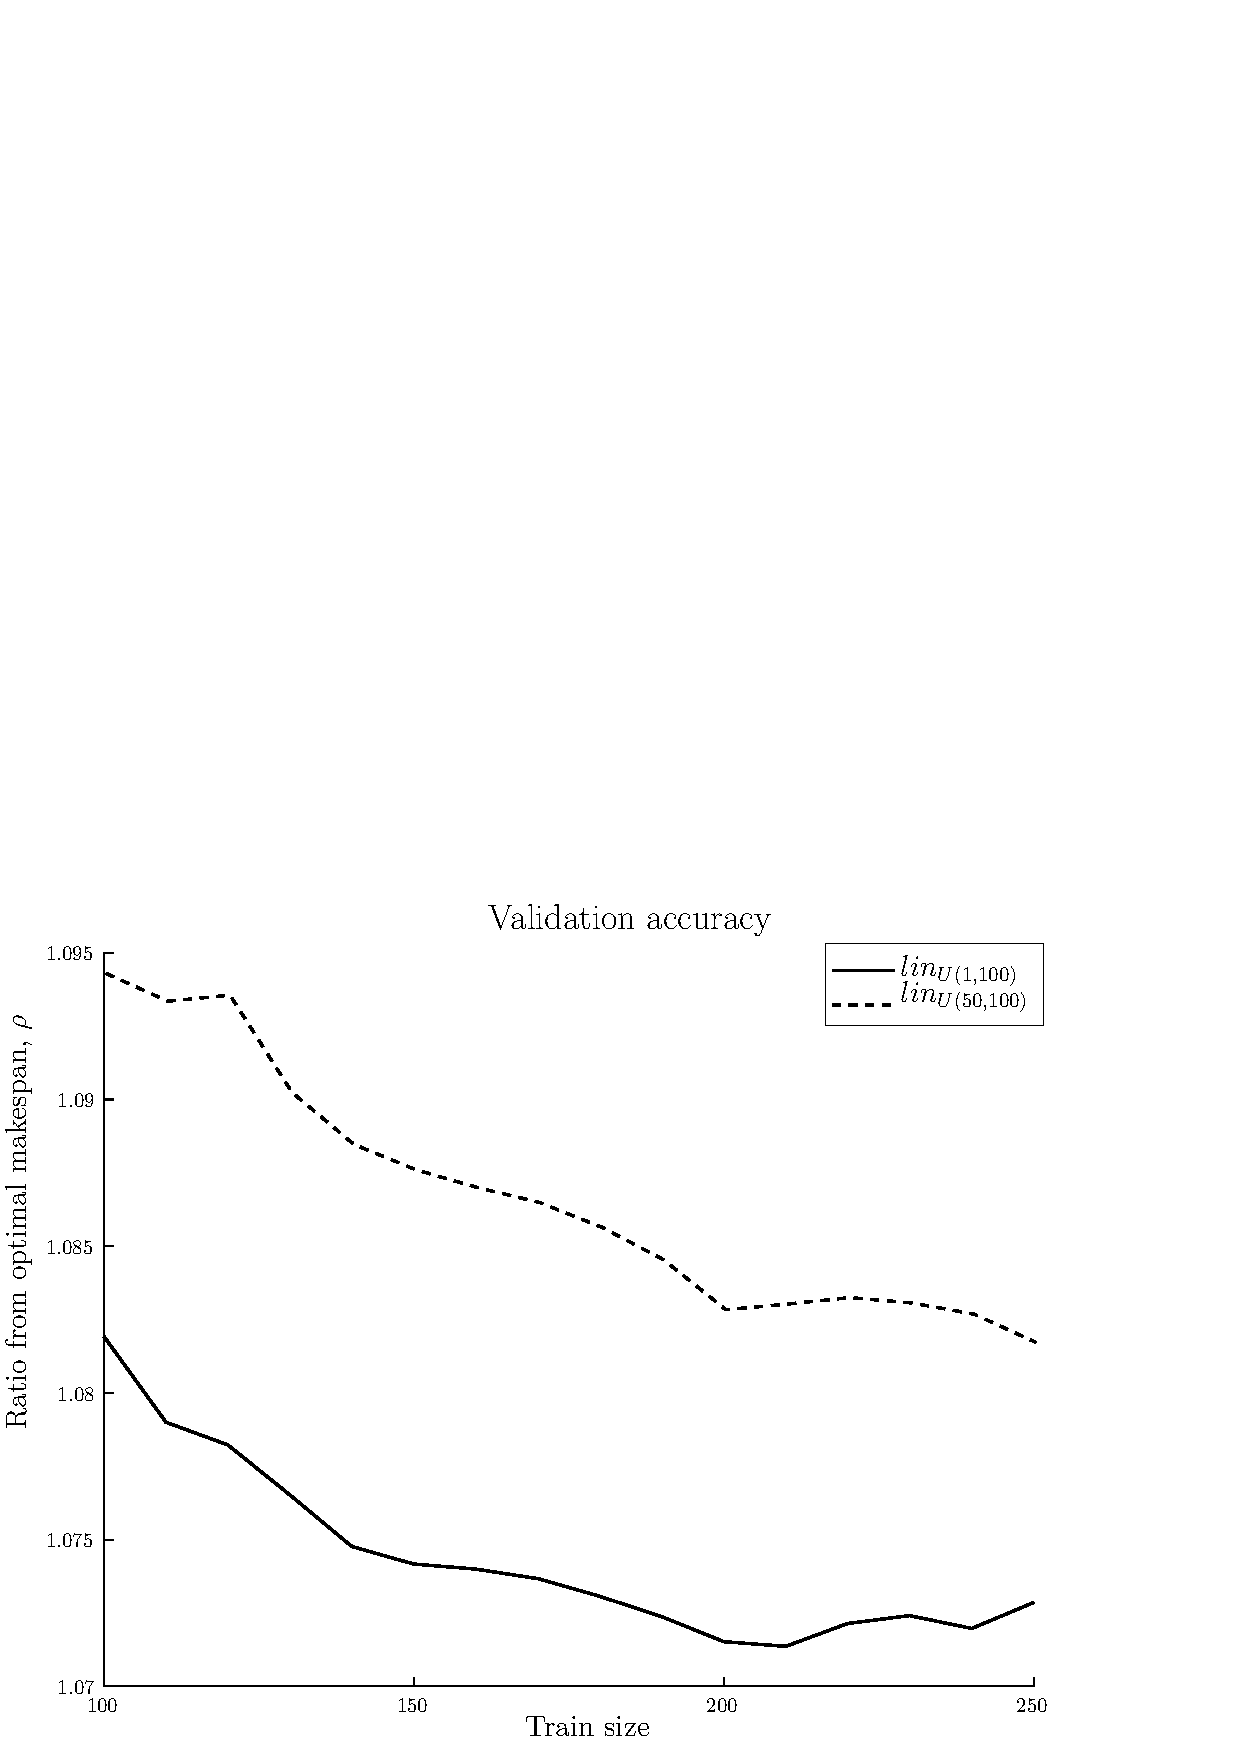
\includegraphics[width=4cm]{../mlb/ordinal/fig1_trainsize.jpg}
\caption{Deviation from optimal makespan as a function of size of training set. Solid line represents model $lin_{U(1,100)}$ and dashed line represents model $lin_{U(50,100)}$.}\end{figure}\end{center}
\end{column}
\end{columns}
}
\frame{\frametitle{Training accuracy}
\begin{center}\begin{figure}[H] 
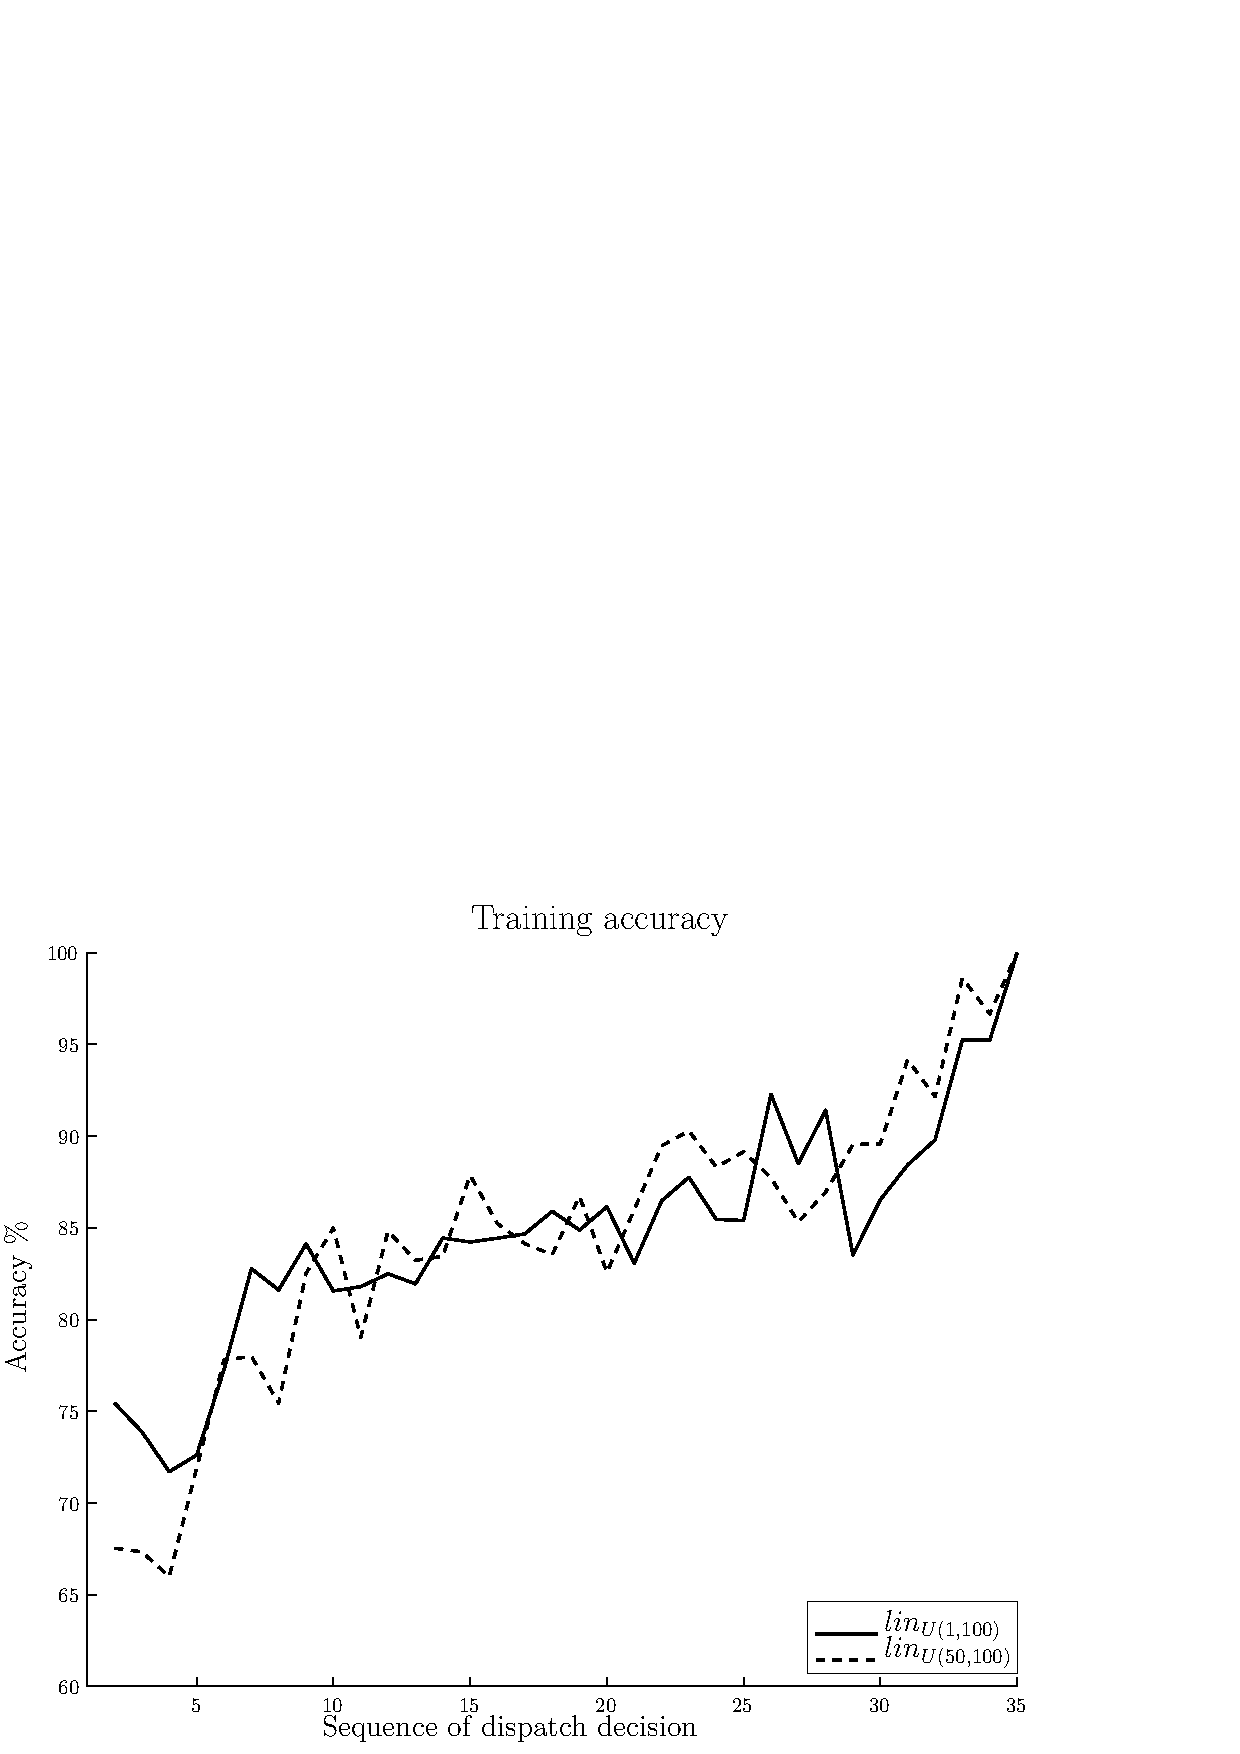
\includegraphics[width=4cm]{../mlb/ordinal/fig2_trainacc.jpg}
\caption{Training accuracy as a function of time. Solid line represents model $lin_{U(1,100)}$ and dashed line represents data distributions $lin_{U(50,100)}$}
\end{figure}\end{center}
}
\subsection{Comparing different dispatching rules}
\frame{\frametitle{Comparing different dispatching rules}
\begin{figure}[t!]
\centering
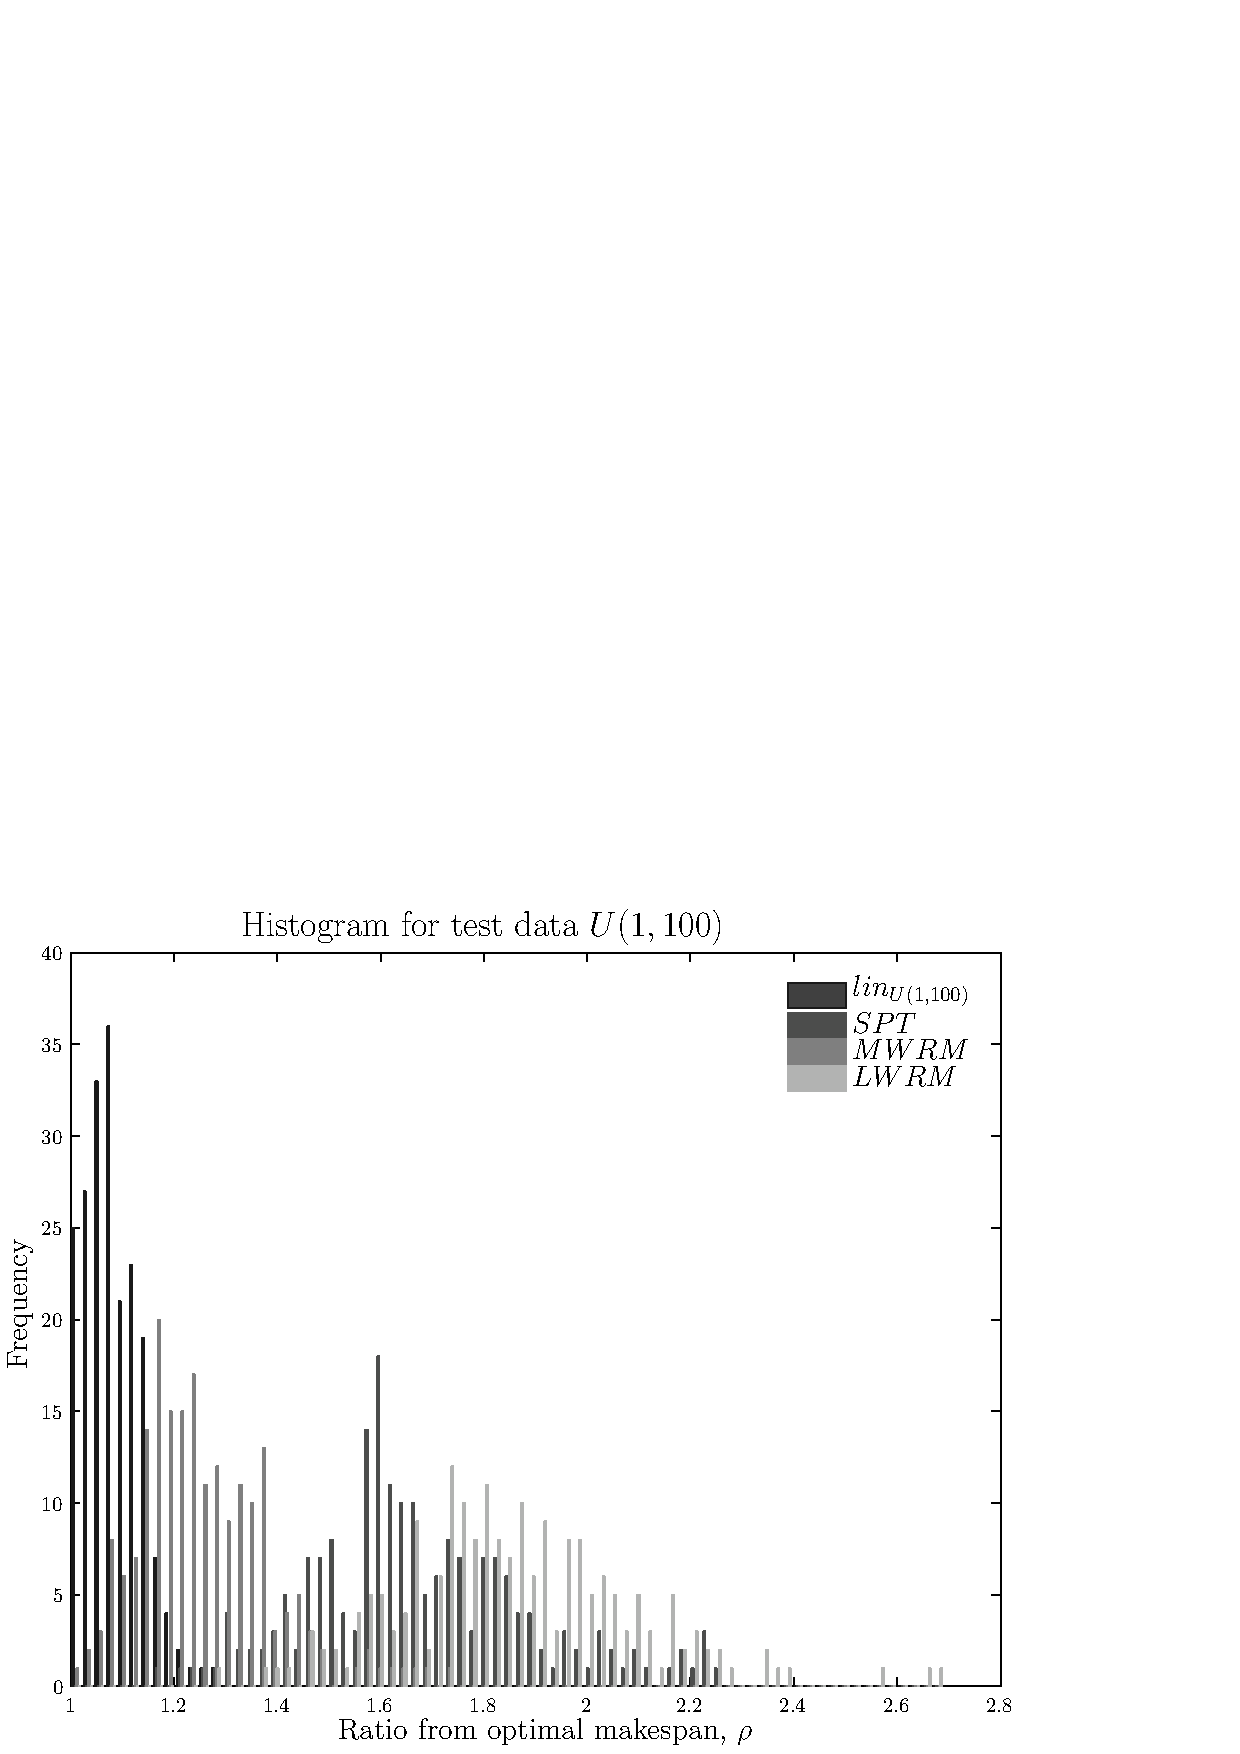
\includegraphics[width=4cm]{../mlb/ordinal/fig3_hist_0_100.jpg}
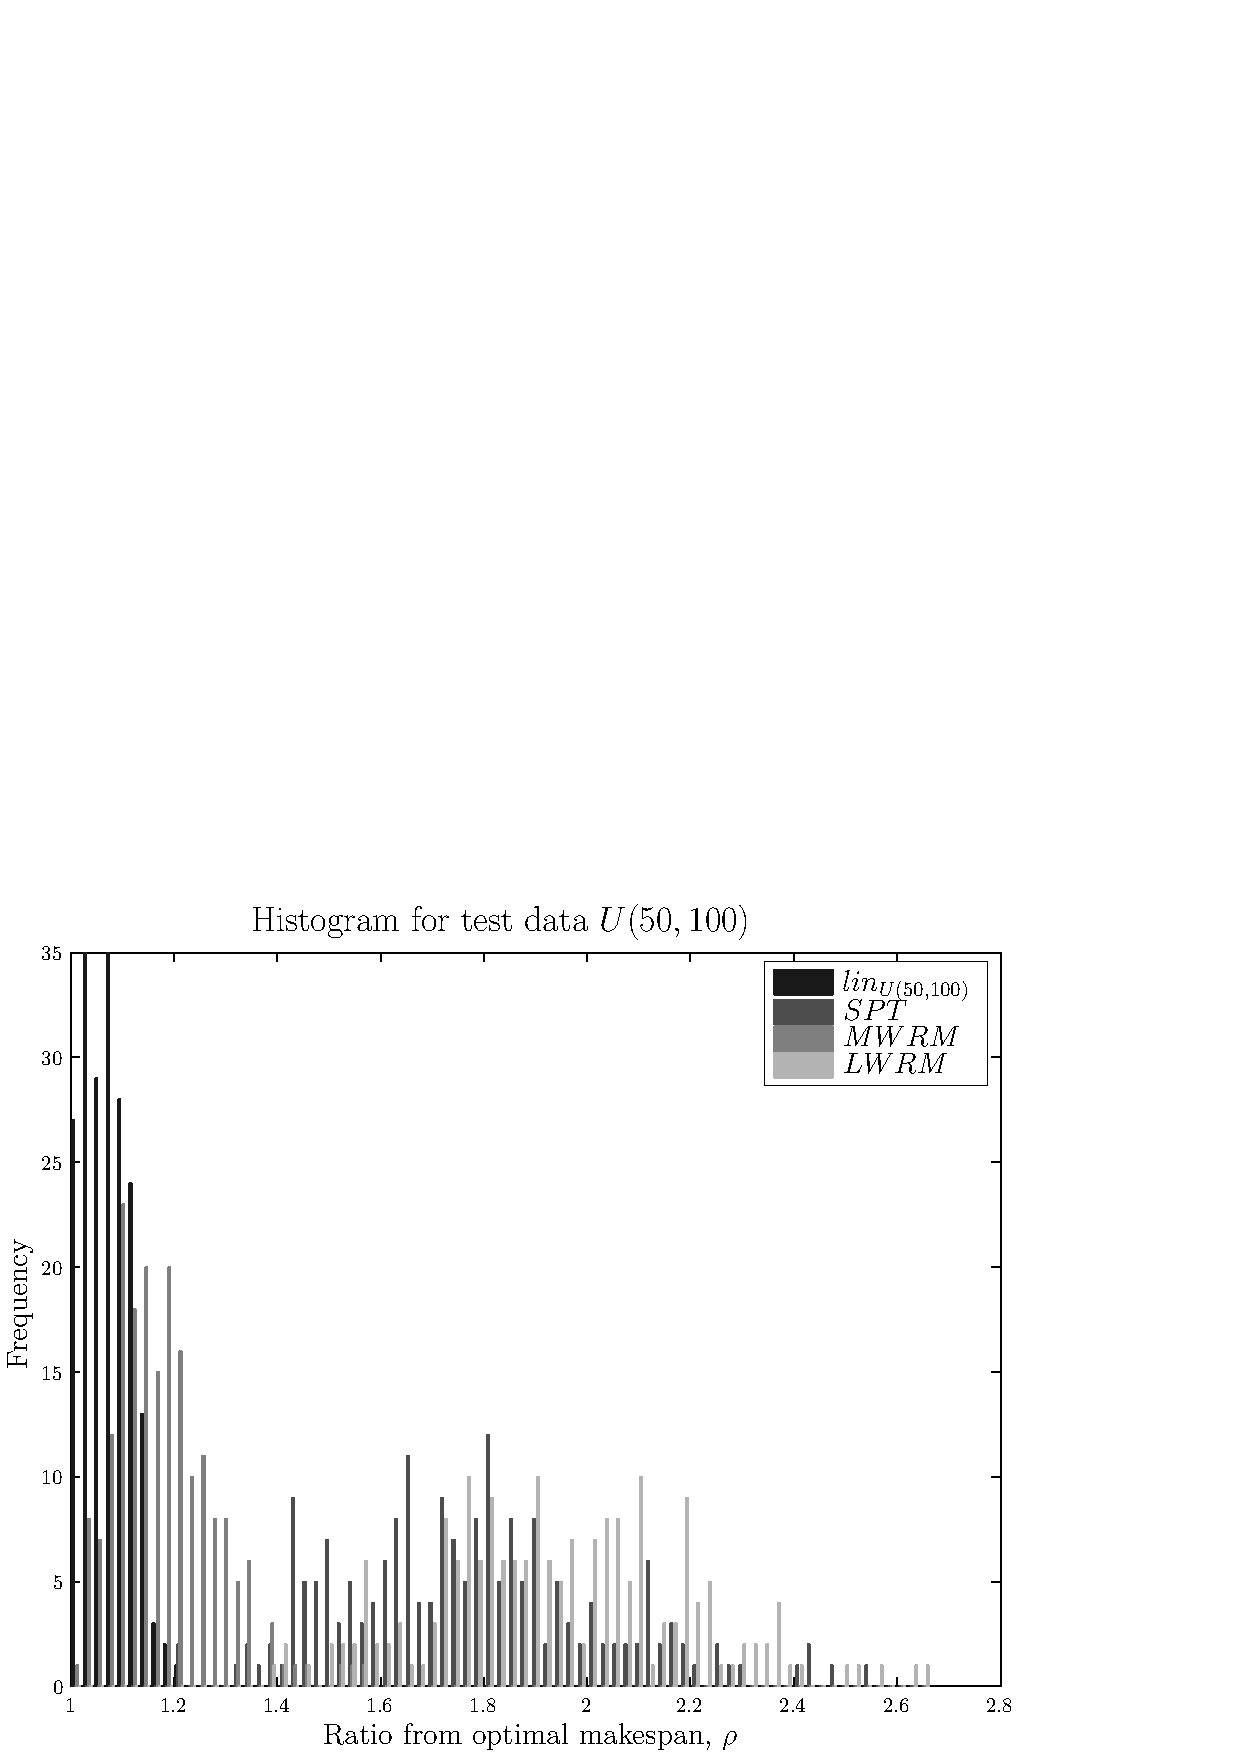
\includegraphics[width=4cm]{../mlb/ordinal/fig3_hist_50_100.jpg}
\caption{Histogram of deviation from optimal makespan for the dispatching rules $(lin_{U(R,100)})$, $(SPT)$, $(MWRM)$ and $(LWRM$). The figure on the left depicts model $lin_{U(1,100)}$, and the figure on the right is of model $lin_{U(50,100)}$.}
\label{fig:densities}
\end{figure}
}
\frame{\frametitle{Comparing different dispatching rules}
\begin{table}[t!]
 {\footnotesize
 \begin{center}
  \begin{tabular}{|p{1.5cm}|ccccc|}
   \hline\hline
   $U(1,100)$ & mean& std    & med    & min    & max   \\ \hline
   $lin_{U(1,100)}$ & 1.0842 & 0.0536 & 1.0785 & 1.0000 & 1.2722\\
   $SPT$     & 1.6707 & 0.2160 & 1.6365 & 1.1654 & 2.2500\\
   $MWRM$    & 1.2595 & 0.1307 & 1.2350 & 1.0000 & 1.7288\\
   $LWRM$    & 1.8589 & 0.2292 & 1.8368 & 1.2907 & 2.6906\\  
   \hline\hline
  \end{tabular}
  \begin{tabular}{|p{1.5cm}|ccccc|}
   \hline\hline
   $U(50,100)$ & mean   & std    & med    & min    & max    \\ \hline
   $lin_{U(50,100)}$    & 1.0724 & 0.0446 & 1.0713 & 1.0000 & 1.2159 \\
   $SPT$         & 1.7689 & 0.2514 & 1.7526 & 1.2047 & 2.5367 \\ 
   $MWRM$        & 1.1835 & 0.0994 & 1.1699 & 1.0217 & 1.5561 \\
   $LWRM$        & 1.9422 & 0.2465 & 1.9210 & 1.3916 & 2.6642 \\ 
   \hline\hline
  \end{tabular}
 \end{center}}
 \caption{Mean value, standard deviation, median value, minimum and maximum values using the test sets corresponding to data distributions $U(1,100)$ (above) and $U(50,100)$ (below) .}
 \label{tbl:stats}
\end{table}
}
\subsection{Robustness towards data distribution}
\frame{\frametitle{Robustness towards data distribution}
\begin{figure}[b!]
\centering
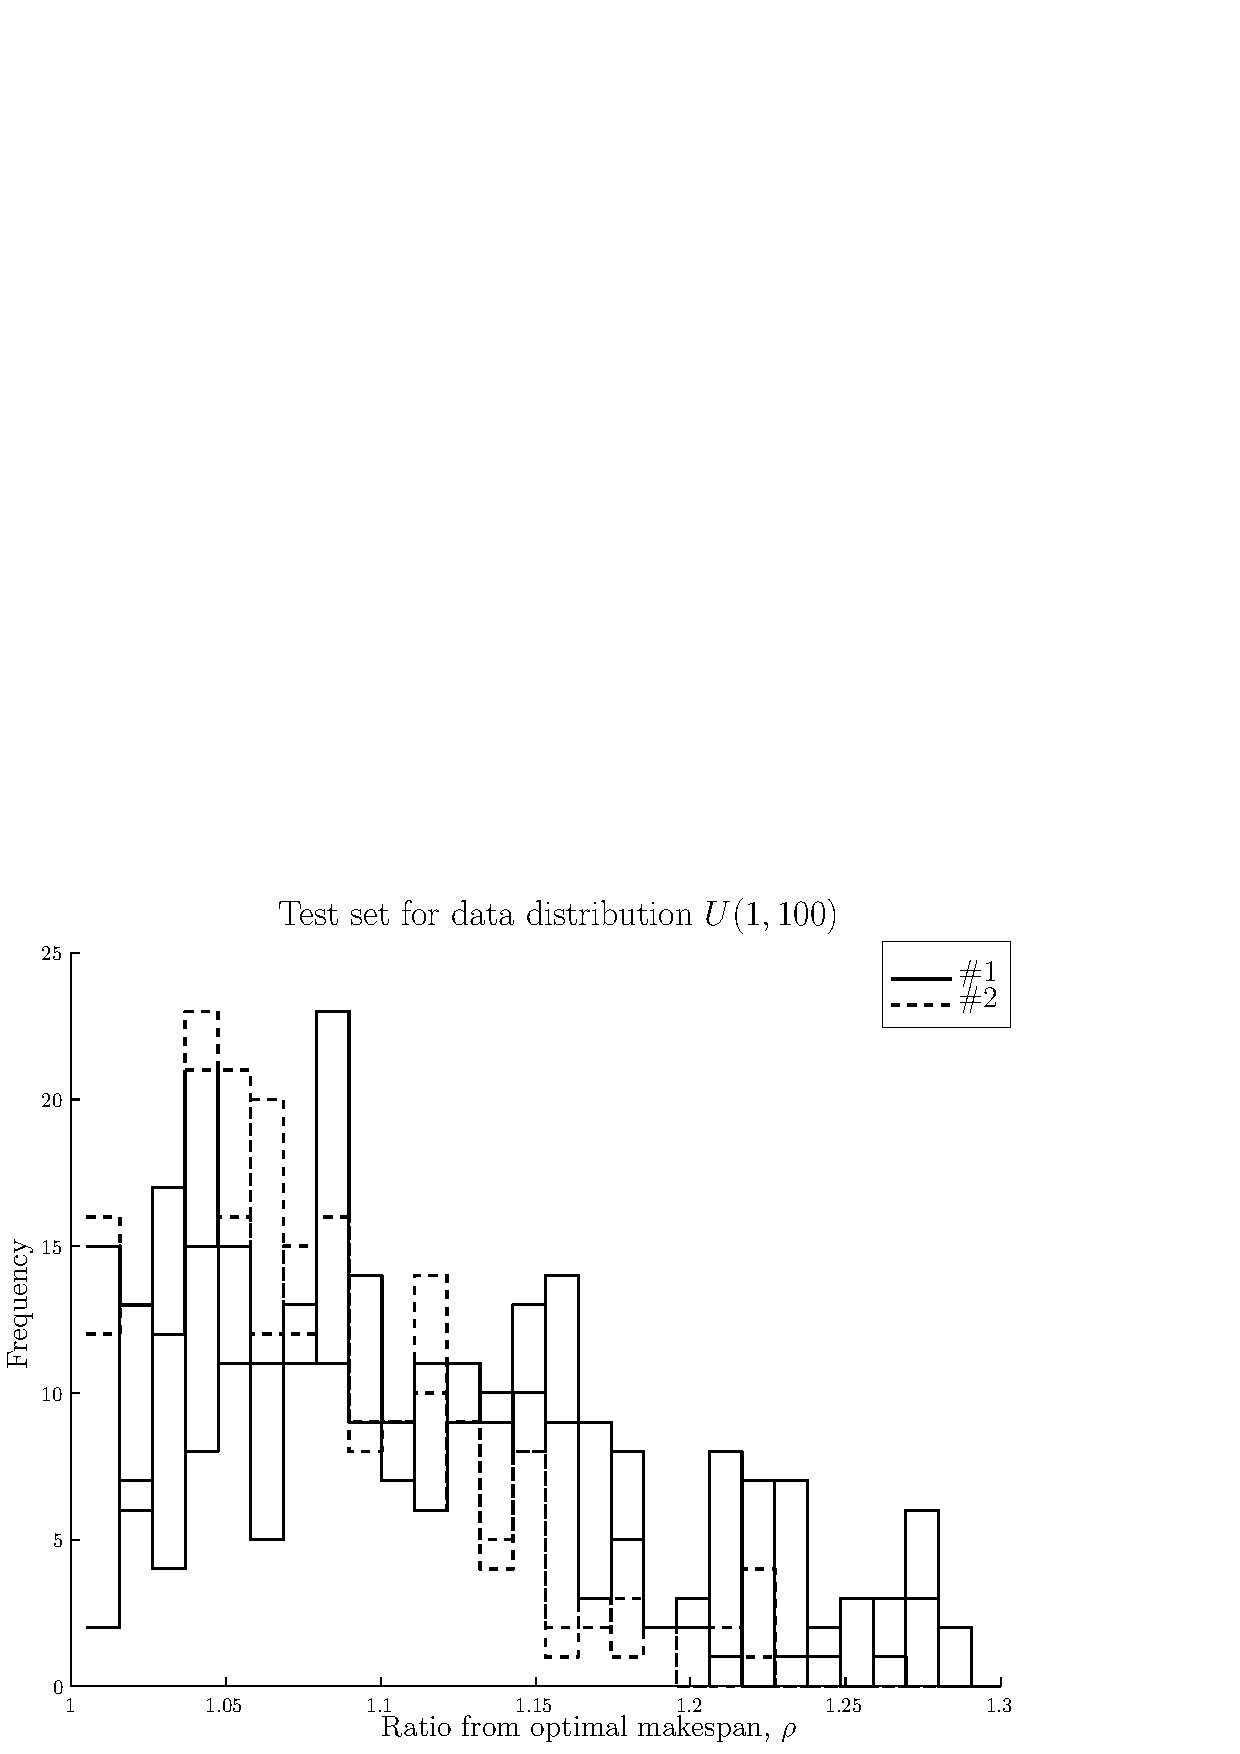
\includegraphics[width=0.4\columnwidth]{../mlb/ordinal/fig4_hist0_100.jpg}
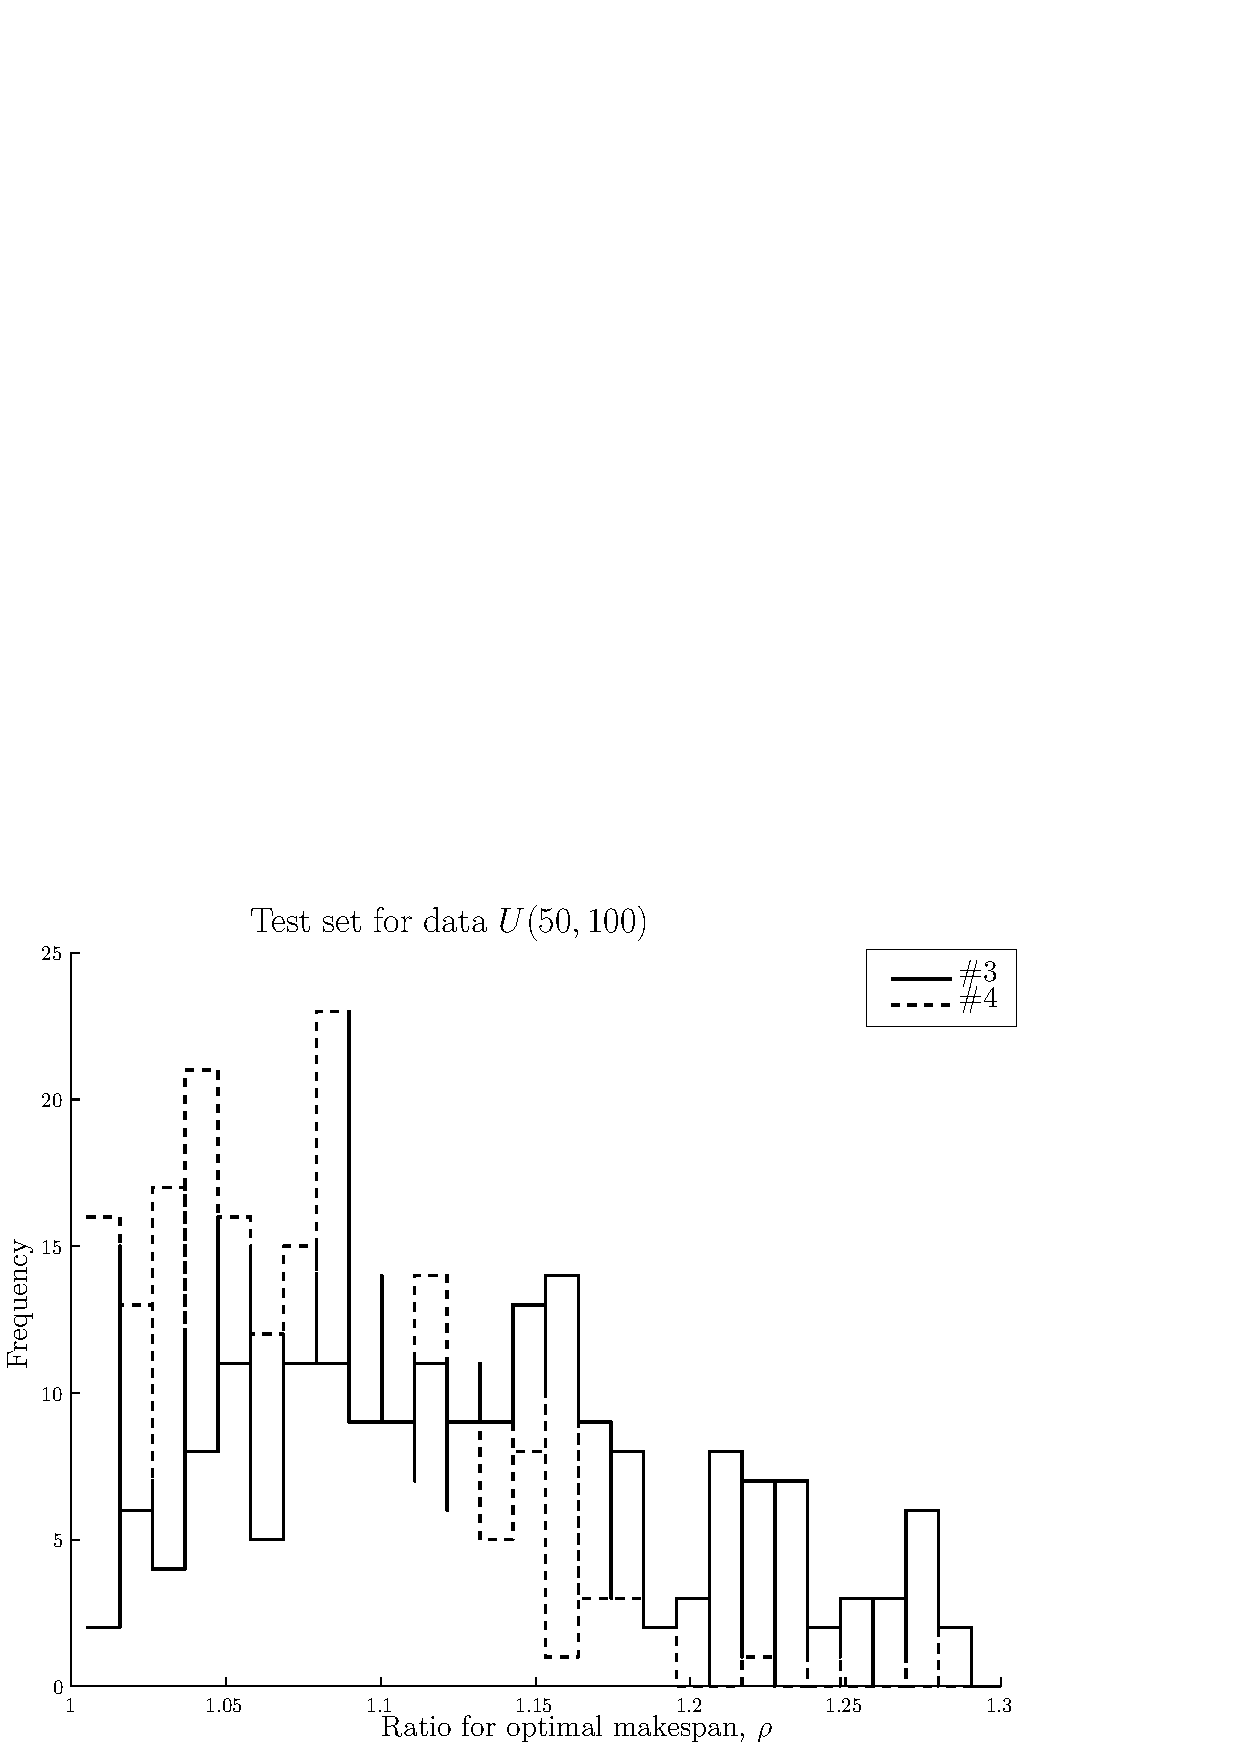
\includegraphics[width=0.4\columnwidth]{../mlb/ordinal/fig4_hist50_100.jpg}
\caption{Histogram of deviation from optimal makespan for the dispatching rules using model trained on either $U(1,100)$ or $U(50,100)$ and tested on both $U(1,100)$ (left) and $U(50,100)$ (right).}
\label{fig:diffdatadistrdensities}
\end{figure}
}
\frame{\frametitle{Robustness towards data distribution}
\begin{table}[h!]
 {\footnotesize
 \begin{center}
  \begin{tabular}{|c|l|l|ccccc|}
   \hline\hline
   & model & test set & mean & std    & med    & min    & max   \\ \hline
\#1 & $lin_{U(1,100)}$ & $U(1,100)$ & 1.0844 & 0.0535 & 1.0786 & 1.0000 & 1.2722  \\
\#2 & $lin_{U(50,100)}$ & $U(1,100)$ & 1.0709 & 0.0497&1.0626 & 1.0000 & 1.2503  \\
\#3 & $lin_{U(1,100)}$ & $U(50,100)$ & 1.1429 & 0.1115&1.1158 & 1.0000 & 1.5963  \\
\#4 & $lin_{U(50,100)}$ & $U(50,100)$ & 1.0724 & 0.0446&1.0713 & 1.0000 & 1.2159  \\
%#4 and #1 are the same distribution
%#4 and #3 are the same distribution
   \hline\hline
  \end{tabular}
 \end{center}}
 \caption{Mean value, standard deviation, median value, minimum and maximum values for the test sets corresponding to data distributions $U(1,100)$ and $U(50,100)$, on both models $lin_{U(1,100)}$ and $lin_{U(50,100)}$.}
 \label{tbl:diffdatadistr}
\end{table}
}
\subsection{Feature selection}
\frame{\frametitle{Feature selection}
\begin{table}[h!]
 {\footnotesize
 \begin{center}
  \begin{tabular}{|c|r|r|p{5cm}|}
   \hline\hline
  weight & $lin_{U(1,100)}$ & $lin_{U(50,100)}$ & description \\ \hline
  $\bar{w}(1)$ &  -0.6712 & -0.2220 & processing time for job on machine\\
  $\bar{w}(2)$ &  -0.9785 & -0.9195 & work remaining \\
  $\bar{w}(3)$ & -1.0549  & -0.9059 & start-time \\
  $\bar{w}(4)$ & -0.7128  & -0.6274 & end-time \\
  $\bar{w}(5)$ & -0.3268  &  0.0103 & when machine is next free \\
  $\bar{w}(6)$ &  1.8678  &  1.3710 & current makespan \\
  $\bar{w}(7)$ & -1.5607  & -1.6290 & slack time for this particular machine \\
  $\bar{w}(8)$ & -0.7511  & -0.7607 & slack time for all machines \\
  $\bar{w}(9)$ & -0.2664  & -0.3639 & slack time weighted w.r.t. number of operations already assigned \\
   \hline\hline
  \end{tabular}
 \end{center}}
 \caption{Mean value, standard deviation, median value, minimum and maximum values for the test sets corresponding to data distributions $U(1,100)$ and $U(50,100)$, on both models $lin_{U(1,100)}$ and $lin_{U(50,100)}$.}
 \label{tbl:features}
\end{table}
}
\frame{\frametitle{Fixed weights vs. varied weights}
\begin{figure}[b!]
\centering
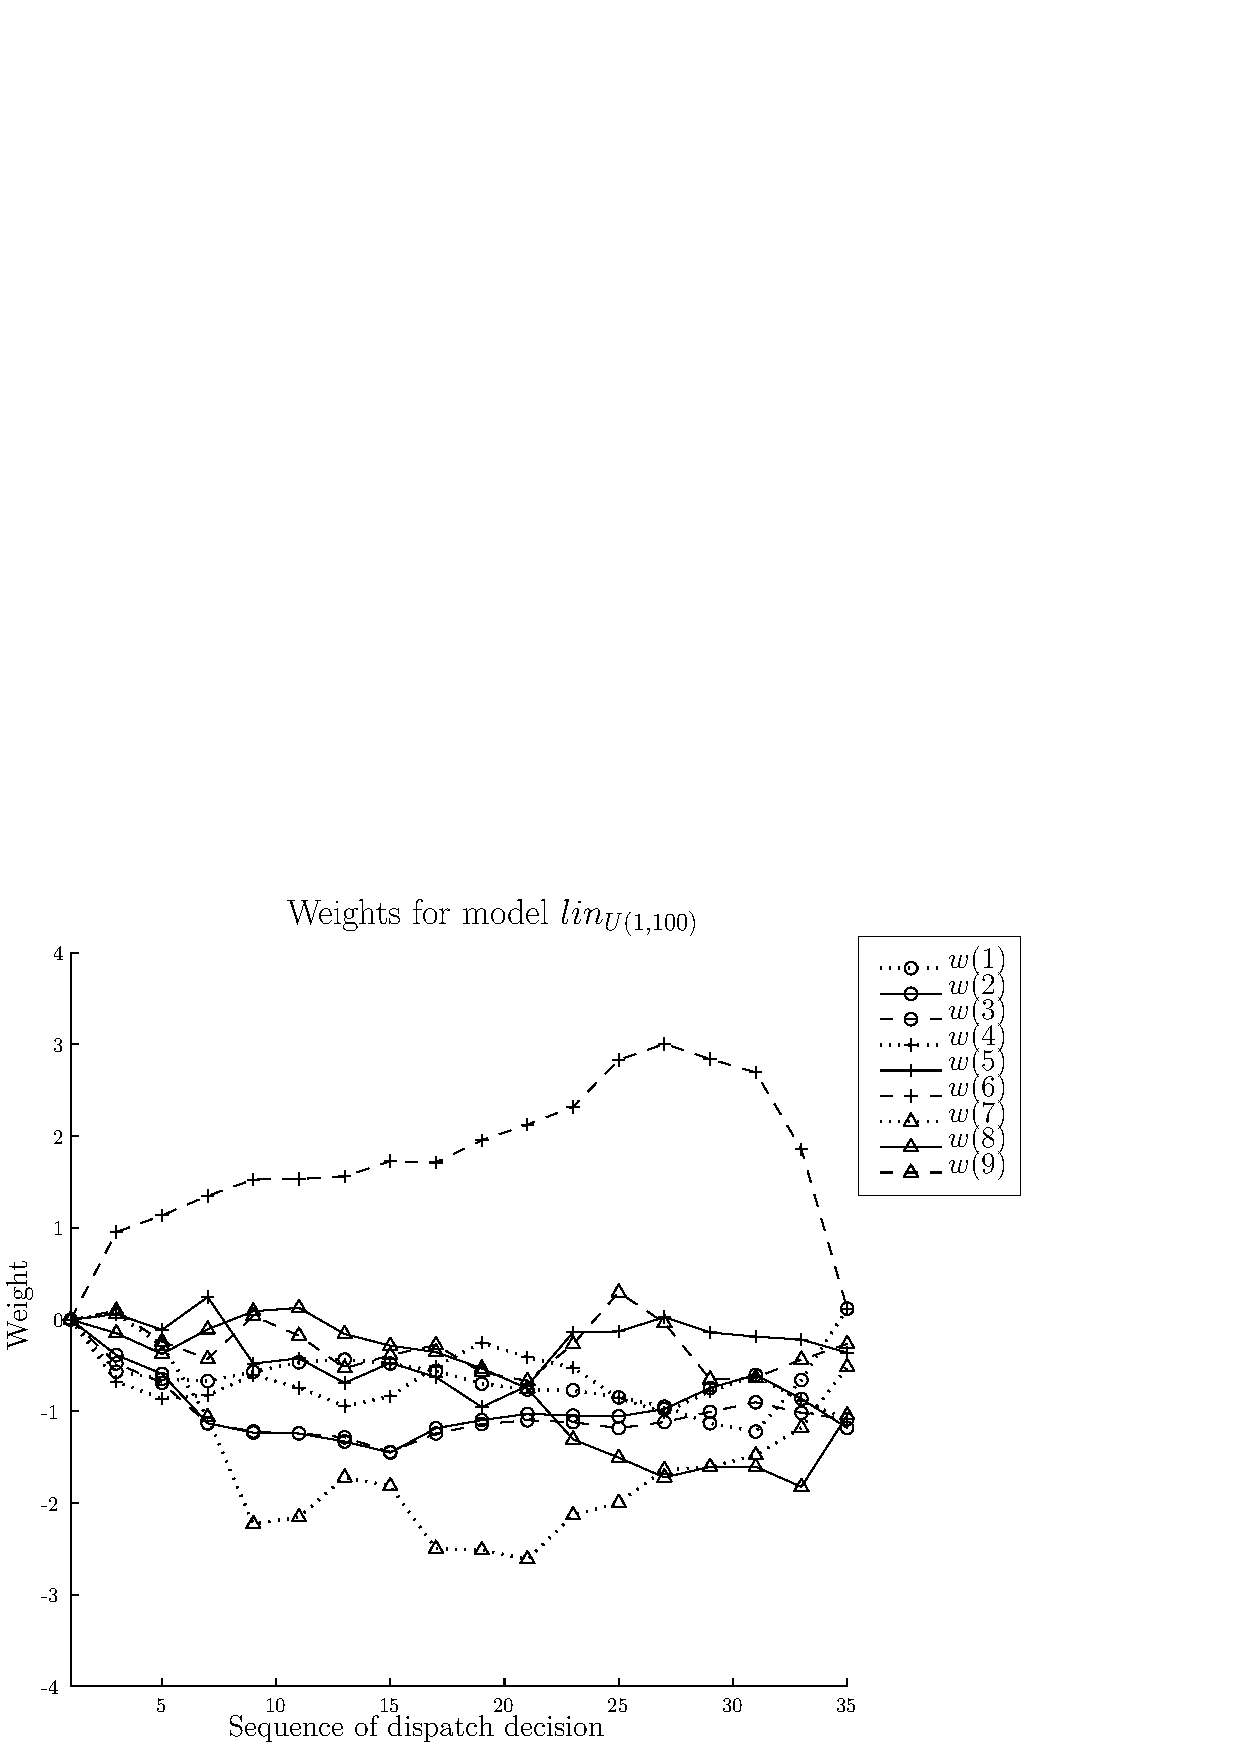
\includegraphics[width=0.45\columnwidth]{../mlb/ordinal/fig6_weights0_100.jpg}
\includegraphics[width=0.45\columnwidth]{../mlb/ordinal/fig6_weights50_100.jpg}
\caption{Weights of features as a function of time, for data distribution $U(1,100)$ (left) and $U(50,100)$ (right).}
\label{fig:variedweights}
\end{figure}
}
\frame{\frametitle{Robustness towards data distribution using fixed weights}
\begin{table}[h!]
 {\footnotesize
 \begin{center}
  \begin{tabular}{|c|l|l|ccccc|}
   \hline\hline
   & model & test set & mean & std    & med    & min    & max   \\ \hline
\#1 & $\bar{lin}_{U(1,100)}$ & $U(1,100)$ & 1.0862 & 0.0580 & 1.0785 & 1.0000 & 1.2722   \\
\#2 & $\bar{lin}_{U(50,100)}$ & $U(1,100)$ & 1.0706 & 0.0493 & 1.0597 & 1.0000 & 1.2204  \\
\#3 & $\bar{lin}_{U(1,100)}$ & $U(50,100)$ &   1.1356 & 0.0791 & 1.1296 & 1.0000 & 1.5284  \\
\#4 & $\bar{lin}_{U(50,100)}$ & $U(50,100)$ &  1.0695 & 0.0459 & 1.0658 & 1.0000 & 1.2201  \\
%#4 and #3 are the same distribution
   \hline\hline
  \end{tabular}
 \end{center}}
 \caption{Mean value, standard deviation, median value, minimum and maximum values for the test sets corresponding to data distributions $U(1,100)$ and $U(50,100)$, on both fixed weight models $\bar{lin}_{U(1,100)}$ and $\bar{lin}_{U(50,100)}$.}
 \label{tbl:diffdatadistr:fixed}
\end{table}
}

\section{Future Work}
{\frame{\frametitle{Future work}
\bi Overcome problems due to non unique sequence representation of JSP
  \item Other learning methods, e.g. reinforcement learning;
  \item Other data distributions and dimensions of JSP
\ei
}
\subsection{References}\frame{\frametitle{References}
\bibliographystyle{alpha}\bibliography{biblio_presentation}
}
\end{document}
%%%%%%%%%%%%%%%%%%%%%%%%%%%%%%%%%%%%%%%
